\section{Digital Certificates}

\subsection{Introduction to Digital Certificates}

\begin{definition}{Digital Certificates}
A digital certificate is a signed statement by a trusted third party (Certificate Authority) that a certain public key belongs to a certain entity (person, organization, or system). Certificates are used to authenticate public keys, not the entities themselves.
\end{definition}

\begin{concept}{Authentication of Public Keys}
The fundamental problem certificates solve is how to reliably distribute public keys in an insecure network:
\begin{itemize}
    \item Without certificates, it's difficult to know if a public key truly belongs to the claimed entity
    \item Certificates bind identities to public keys through the endorsement of a trusted third party
    \item The binding is authenticated through cryptographic signatures
\end{itemize}
\end{concept}

\begin{definition}{Certificate Types}
Different certificate types serve different purposes:
\begin{itemize}
    \item \textbf{TLS Certificates}:
    \begin{itemize}
        \item Domain Validation (DV) - Validates domain ownership only
        \item Organization Validation (OV) - Validates domain ownership and organization details
        \item Extended Validation (EV) - Provides the highest level of validation
    \end{itemize}
    \item \textbf{Code signing certificates} - Authenticate software and files
    \item \textbf{Client certificates} - Identify individual users or machines
\end{itemize}
\end{definition}

\begin{concept}{PKI} Public Key Infrastructure:
    Verify public key in the certificate by verifying the signature
\end{concept}


\subsection{X.509 Certificate Structure}

\begin{definition}{X.509 Standard}
X.509 is the dominant certificate standard, developed by the International Telecommunication Union (ITU). X.509 certificates are described in ASN.1 notation and typically encoded using DER (Distinguished Encoding Rules).
\end{definition}

\begin{concept}{X.509 Certificate Fields}
Key components of an X.509 certificate include:
\begin{itemize}
    \item \textbf{Version} - Certificate format version (v1, v2, or v3)
    \item \textbf{Serial Number} - Unique identifier assigned by the issuing CA
    \item \textbf{Signature Algorithm ID} - Algorithm used to sign the certificate
    \item \textbf{Issuer Name} - X.500 Distinguished Name of the issuing CA
    \item \textbf{Validity Period} - Start and end dates for certificate validity
    \item \textbf{Subject Name} - X.500 Distinguished Name of the certificate owner
    \item \textbf{Subject Public Key Info} - The public key and algorithm identifier
    \item \textbf{Extensions} - Additional fields (e.g., key usage, alternative names)
    \item \textbf{Certificate Signature} - The digital signature created by the CA
\end{itemize}
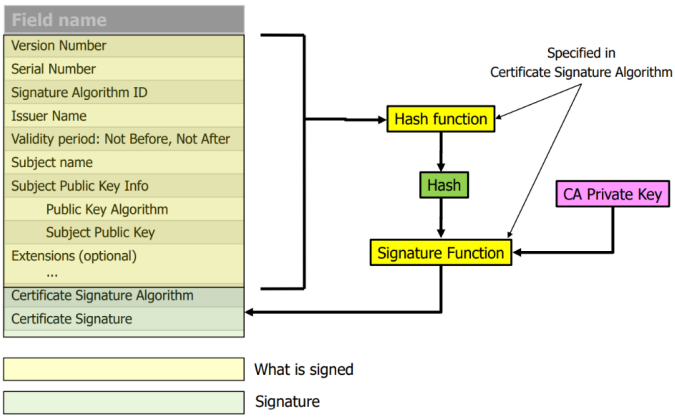
\includegraphics[width=0.7\linewidth]{x509.png}
\end{concept}

\subsection{Certificate Chains and Trust}

\begin{concept}{Certificate Chains}
Certificates form chains of trust:
\begin{itemize}
    \item \textbf{End entity certificates} - Used by servers, clients, or devices
    \item \textbf{Intermediate CA certificates} - Issued by root CAs to intermediate CAs
    \item \textbf{Root CA certificates} - Self-signed certificates from trusted root authorities
\end{itemize}
To verify a certificate, each certificate in the chain must be validated up to a trusted root.
\end{concept}

\begin{formula}{Certificate Chain Validation}
    For $i = [1, n - 1]$
    \begin{itemize}
        \item $C[i].issuer = C[i + 1].subject$
        \item $C[i].signature$ can be verified with $C[i + 1].publicKey$
    \end{itemize}
\end{formula}

\begin{lemma}{Certificate Validation Process}\\
To validate a certificate chain of length n with certificates C[1], ..., C[n], where C[1] is the end entity certificate:
\begin{enumerate}
    \item Check that C[1].name matches the expected entity name
    \item For i = 1 to n - 1:
    \begin{itemize}
        \item Check that C[i].issuer = C[i+1].subject
        \item Verify C[i].signature using C[i+1].publicKey
    \end{itemize}
    \item Locate root cert R with C[n].issuer = R.subject
    \item Verify C[n].signature using R.publicKey
    \item Verify R.signature using R.publicKey (self-verification)
\end{enumerate}
\end{lemma}

\begin{theorem}{Root Certificate Trust}\\
Root certificates are the foundation of trust in PKI:
\begin{itemize}
    \item Root certificates are pre-installed in operating systems and browsers
    \item They're the ultimate trust anchors that enable the validation of all other certificates
    \item The security of PKI depends on the protection of root CA private keys
\end{itemize}
\end{theorem}



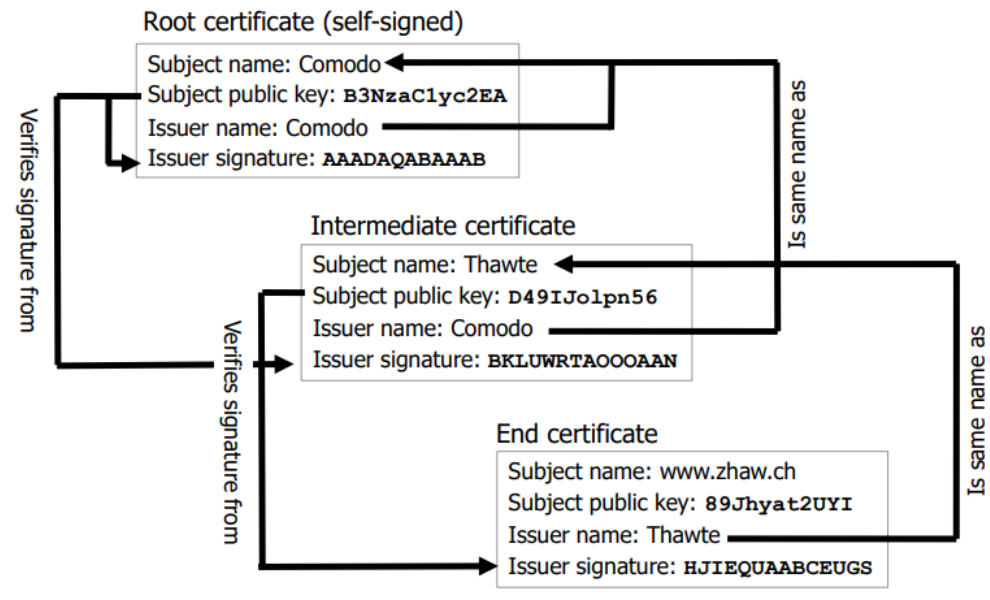
\includegraphics[width=0.7\linewidth]{certificate_chain.png}




\subsection{Root Certificates}

\begin{concept}{Root Certificates}
    Any certificate chain ends with a root certificate.
    \begin{itemize}
        \item Can be verified with its own public key
        \item Root certificates are always self-signed
        \item Usually stored in your browser (from trusted parties)
    \end{itemize}
\end{concept}

\begin{concept}{Root CA Revocation}
    \begin{itemize}
        \item Remove root CA from applications and systems
        \item All certificate issue by the root CA will also be invalid
    \end{itemize}
\end{concept}

\subsection{Validation}

\begin{KR}{Certificate Validation Process}

    \textbf{Step 1} Obtain and verify (validity) root certificate

    \textbf{Step 2} Verify server certificate signature with root public key

    \textbf{Step 3} Compare root certificate subject with server issuer
\end{KR}





\subsection{Certificate Revocation}

\begin{definition}{Certificate Revocation}\\
Certificate revocation is the process of invalidating a certificate before its expiration date, typically due to:
\begin{itemize}
    \item Compromise of the associated private key
    \item Change in the certificate owner's status
    \item Cessation of operation by the certificate owner
\end{itemize}
\end{definition}

\begin{concept}{Certificate Revocation Mechanisms}\\
Several mechanisms exist for checking certificate revocation status:
\begin{itemize}
    \item \textbf{Certificate Revocation Lists (CRLs)} - Lists of revoked certificates published by CAs
    \item \textbf{Online Certificate Status Protocol (OCSP)} - Protocol for real-time certificate status checking
    \item \textbf{OCSP Stapling} - Server includes pre-fetched OCSP response during TLS handshake
    \item \textbf{OCSP Must-Staple} - Requires OCSP stapling for a certificate to be considered valid
    \item \textbf{Browser-Summarized CRLs} - Browser vendors compile and compress CRLs for distribution to browser instances
\end{itemize}
\end{concept}

\begin{KR}{Checking Certificate Revocation}
\paragraph{Using CRLs}
\begin{itemize}
    \item Retrieve CRL from the URL specified in the certificate
    \item Verify CRL signature using the issuing CA's public key
    \item Check if the certificate's serial number appears in the CRL
\end{itemize}

\paragraph{Using OCSP}
\begin{itemize}
    \item Send HTTP request to the OCSP responder URL in the certificate
    \item Include certificate serial number in the request
    \item Receive signed response indicating certificate status (good, revoked, unknown)
    \item Verify signature on the response using the issuing CA's public key
\end{itemize}

\paragraph{Using OCSP Stapling}
\begin{itemize}
    \item Server periodically requests OCSP status from the CA
    \item Server caches the signed OCSP response
    \item Server includes the response in the TLS handshake
    \item Client verifies the OCSP response signature using the CA's public key
\end{itemize}
\end{KR}

\subsection{Certificate Transparency}

\begin{concept}{Certificate Transparency}
Certificate Transparency (CT) is a framework designed to detect and prevent the fraudulent issuance of certificates:
\begin{itemize}
    \item Publicly auditable logs of all issued certificates
    \item Monitors check logs for suspicious certificates
    \item Browsers require evidence that certificates are logged
    \item Helps detect malicious or mistakenly issued certificates
\end{itemize}
\end{concept}

\begin{example}
Let's Encrypt, a free and automated Certificate Authority, has become the largest CA with over 234 million active certificates. It uses the ACME (Automatic Certificate Management Environment) protocol to automate the validation, issuance, and renewal of certificates. Let's Encrypt provides only Domain Validation (DV) certificates with a validity period of 90 days, encouraging frequent renewal and automation.
\end{example}


\subsection{Online Certificate Status Protocol - OCSP}

\mult{2}

\begin{definition}{OCSP}\\
    Issuing CA can be asked (Client) for the status of a specific certificate.
    \begin{itemize}
        \item Status information is updated more often
        \item Only little information is exchanged
        \item OCSP must always be available
        \item OCSP is the single point of failure
        \item Vulnerable to DoS attack against OCSP
    \end{itemize}
    
    Most clients implement soft fail (good), if the response is not received (in time).

    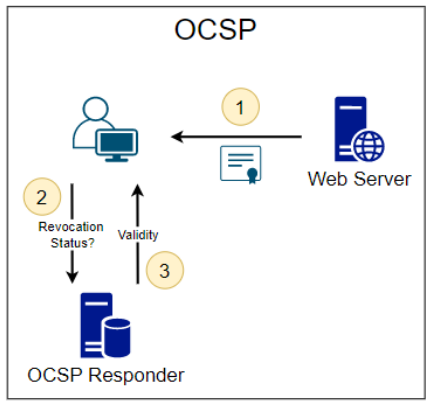
\includegraphics[width=\linewidth]{OCSP.png}
\end{definition}



\begin{concept}{OCSP Stapling}\\
    The server queries the OCSP-Responder listed in the certificate itself and caches the responses.
    \begin{itemize}
        \item Client gets OCSP response from server during TLS handshake
        \item Less dependent on the availability of OCSP-Responder
    \end{itemize}
    
    \textbf{Limitations}
    \begin{itemize}
        \item Vulnerable time window like in CRL
        \item Fallback to OCSP if no valid response is cached
    \end{itemize}

    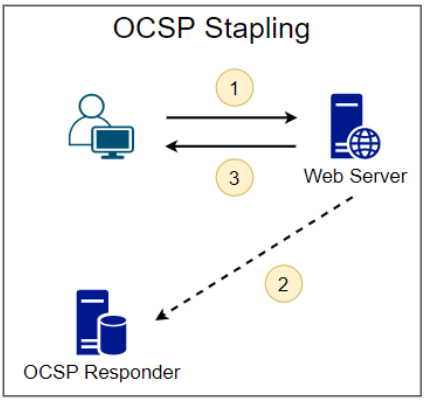
\includegraphics[width=\linewidth]{OCSP_stapling.png}
\end{concept}

\multend
